%!TEX root = ../INTO-CPS-Manifesto.tex

\newcommand{\CML}{\textsf{CML}}

\section{The INTO-CPS Foundations}\label{sec:foundations}

%\fbox{Jim Woodcock}

%\fbox{JCPW: Add a short introduction}

The development of tools and methods in INTO-CPS is based on a sound semantic description of co-simulation. Our tools use VDM-RT as the discrete-event language and Modelica as the continuous-time language. The framework for co-simulation is based on FMI. We have formalised and mechanised both languages in this framework using Isabelle/UTP. We have a semantics of the relevant parts of SysML that can be used with FMI. These foundations allow for the formal checking of the validity of analysis and co-simulation results. The value of the foundational tools, with both theorem proving and model checking, have been demonstrated to add value to the INTO-CPS tool chain.

\subsection{Foundations of the SysML profile for CPS modelling}

The INTO-CPS project proposes a novel technique for proof-based analysis of co-simulations that considers both architectural and behavioural properties of co-simulations. In D2.3a~\cite{INTO-CPS-D2.3a-2017}, the technique is illustrated by way of two case studies, one from from railways and another one from the area of smart buildings control. D2.2a~\cite{INTO-CPS-D2.2a-2016} instantiates the approach to robotic control.

\subsubsection{SysML}

The Systems Modelling Language (SysML)~\cite{OMGSysML2012} builds on the Unified Modelling Language (UML) to provide a general-purpose notation for systems engineering. SysML supports the modelling of CPSs, which are designed to actively engage with the physical world in which they reside. They tend to be heterogeneous: their subsystems tackle a wide variety of domains (such as, mechanical, hydraulic, analogue, and a plethora of software domains) that mix phenomena of both continuous and discrete nature, typical of physical and software systems, respectively. Such systems are typically engineered using a variety of languages and tools that adopt complementary paradigms; examples are physics-related models, control laws, and sequential, concurrent, and real-time programs. This diversity makes CPS generally difficult to analyse and study.

\subsubsection{Co-simulation}

CPSs are often handled modularly to tackle this heterogeneity and complexity. To separate concerns effectively, the global model of the system is decomposed into subsystems, each typically focused on a particular phenomenon or domain and tackled by the most appropriate modelling technique. Simulation, the standard validation technique for CPS, is often carried out modularly also, using co-simulation~\cite{GomesTBLV2017,Gomes&18}, the coupling of subsystem simulations. This constitutes the backdrop of the industrial Functional Mockup Interface (FMI) standard~\cite{FMIStandard2014,BromanBGLMTW2013,CavalcantiWA16} for co-simulation of components built using distinct modelling tools. The FMI Standard has been proposed to address the challenge of interoperability, coupling different simulators and their high-level control components via a bespoke FMI API.

While co-simulation is currently the predominant approach to analyse CPS, INTO-CPS proposes a proof-based complementary technique that uses mathematical reasoning and logic. Simulation is useful in helping engineers to understand modelling implications and spot design issues, but cannot provide universal guarantees of correctness and safety. It is usually impossible to run an exhaustive number of simulations as a way of testing the system. For these reasons, it is often not clear how the evidence provided by simulations is to be qualified, since simulations depend on parameters and algorithms, and are software systems (with possible faults) in their own right.

Proof-based techniques, on the other hand, hold the promise of making universal claims about systems. They can potentially abstract from particular simulation scenarios, parametrisations of models, and interaction patterns used for testing. In traditional software engineering, they have been successfully used to validate the correctness of implementations against abstract requirements models~\cite{WoodcockLBF2009}. Yet, their application to CPS is fraught with difficulties: the heterogeneous combination of languages used in typical descriptions of CPS raises issues of semantic integration and complexity in reasoning about those models. The aspiring ideal of any verification technique is a compositional approach, and such approaches are still rare for CPS~\cite{NuzzoLFS2018}.

\subsubsection{The INTO-CPS approach to verification and co-simulation}

Our approach is to formally verify the well-formedness and healthiness of SysML CPS architectural designs as a prelude to co-simulation. The designs are described using INTO-SysML~\cite{INTO-CPS-D2.1a-2015}, a profile for multi-modelling and FMI co-simulation. The well-formedness checks verify that designs comply with all the required constraints of the INTO-SysML meta-model; this includes connector conformity, which checks the adequacy of the connections between SysML blocks (denoting components) with respect to the types of the ports being wired. The healthiness checks concern detection of algebraic loops, a feedback loop resulting in instantaneous cyclic dependencies; this is relevant because a desirable property of co-simulation, which often reduces to coupling of simulators, is convergence (where numerical analyses approximate the solution), which is dependent on the structure of the subsystems and cannot be guaranteed if this structure contains algebraic loops~\cite{KublerS2000,BromanBGLMTW2013}. The work in the INTO-CPS project demonstrates the capabilities of our verification workbench for modelling languages and engineering theories mechanised in the Isabelle proof assistant~\cite{NipkowK2014}, and the CSP process algebra~\cite{Hoare1985} with its accompanying FDR3 refinement-checker~\cite{GibsonRobinsonABR2016}.

Our technique is based on abstraction: we use a relational view of FMUs that abstracts from reactive behaviours as well as the API imposed by FMI. This allows us to focus on the fundamental properties of a co-simulation, while introducing details into the model view refinement that preserves those properties.

\subsubsection{Instantiation for robotics applications}

We have extended and restricted the INTO-SysML profile to deal with mobile and autonomous robotic systems. For modelling the controllers, we use RoboChart~\cite{LiMRCWT2017}. For modelling the robotic platform and the environment, we use Simulink~\cite{MathworksURL}. We have also given a behavioural semantics for models written in the profile using CSP. The semantics is agnostic to RoboChart and Simulink, and captures a co-simulation view of the multi-models based on the FMI API.

Our semantics can be used in two ways. First, by integration with a semantics of each of the multi-models that defines their specific responses to the simulation steps, we can obtain a semantics of the system as a whole. Such semantics can be used to establish properties of the system, as opposed to properties of the individual models. In this way, we can confirm the results of co-simulations via model checking or theorem proving, for example.

There are CSP-based formal semantics for RoboChart~\cite{MiyazawaCRLWT2016} and Simu\-link~\cite{MarriottZC2012,CavalcantiMW2013} underpinned by a precise mathematical semantics. Our next step is their lifting to provide an FMI-based view of the behaviour of models written in these notations. With that, we can use RoboChart and Simulink models as FMUs in a formal model of a co-simulation as suggested here, and use CSP and its semantics to reason about the co-simulation.

It is also relatively direct to wrap existing CSP semantics for UML state machines~\cite{DaviesC2003,RaschW2005} to allow the use of such models as FMUs in a co-simulation. In this case, traditional UML modelling can be adopted.

Secondly, we can use our semantics as a specification for a co-simulation. The work in~\cite{CavalcantiWA16} provides a CSP semantics for an FMI co-simulation; it covers not only models of the FMUs, but also a model of a master algorithm of choice. The scenario defined by an INTO-SysML model identifies inputs and outputs, and their connections. The traces of the FMI co-simulation model should be allowed by the CSP semantics of the INTO-SysML model.

There is no support to establish formal connections between a simulation and the state machine and physical models (of the robotic platform and the environment). The SysML profile proposed here supports the development of design models via the provision of domain-specific languages based on familiar diagrammatic notations and facilities for clear connection of models. Complementarily, as explained above, the semantics of the profile supports the verification of FMI-based co-simulations.  There are plans for automatic generation of simulations of RoboChart models~\cite{CavalcantiWA16}. The semantics we propose can be used to justify the combination of these simulations with Simulink simulations as suggested above.

\subsubsection{Future work}

We first suggest the development of a tool that supports the user of our technique in automatically generating the Isabelle/UTP architectural model, as well as a sketch of the behavioural model. The formal developer can use the sketch as a starting point, completing it with a detailed encoding of functional behaviours of FMUs. Secondly, elements of the refinement strategy from abstract into concrete FMU models ought be explored for a larger spectrum of case studies and examples, beyond the ones we presented in this report. Both these works could be tackled by the INTO-CPS Association.

INTO-CPS multi-models are composed of individual models whose foundations lie in a variety of modelling notations, each of which has its own unique syntax, semantics, and underlying paradigmatic concepts, such as discrete or continuous time.  The purpose of a multi-model is to assign behaviour to a CPS by composing the behaviours of the constituent models.  Thus, in order to provide an integrated tool chain for trustworthy CPS development, there is a necessity for unification of these underlying semantic models to allow consistent integration of heterogeneous system components.  This will then allow us to substantiate statements made about the multi-model with respect to the underlying mathematical core.  Hoare and He's UTP~\cite{Hoare&98} has been designed as a framework in which the integration of languages, through the common semantic domain of the alphabetised relation calculus, can be achieved.  In the next two sections, we describe how UTP is used to provide the foundations for continuous-time modelling in the INTO-CPS tool chain.

\subsection{Discrete Event Models}

VDM-RT is a real-time dialect of the VDM formal modelling language that can be applied to the specification of discrete controllers for CPSs.  VDM-RT is object oriented, where all models are defined as classes that are instantiated as objects.  It supports concurrency through threading and communication between threads through shared objects.  The real-time features of the language comprise abstractions for deployment of objects to computing units that are connected by buses, and the time taken to evaluate expressions that advance a global ``wall clock'' to predict the computation time of a model.

A denotational semantics exists for the core specification language~\cite{Larsen&95c}, and a structured operational semantics (SOS) exists for the real-time aspects~\cite{Lausdahl&13a}, but there is currently no full semantic description of VDM-RT.  To address this, the INTO-CPS project has established a comprehensive denotational semantics for the VDM-RT language, including object orientation, real time, and concurrency.

We have given a UTP semantics to the language, and mechanised this in the Isabelle/UTP theorem prover.  The basis for our treatment of object orientation is an extended calculus for classes and objects, including novel healthiness conditions that allow handling of multiple inheritance.  Our semantics includes a new approach to handling static attributes, methods, and constructors.  We have mechanised Lausdahl's operational semantics of VDM-RT~\cite{Lausdahl&13a} in Isabelle/HOL, which allowed us to gain greater insight into the language.

We use UTP~\cite{Hoare&98,Cavalcanti&06} to give a denotational semantics to VDM-RT.  VDM-RT is a discrete real-time language, which leads us to employ the UTP theory of timed reactive designs as the semantic model, as embodied in the COMPASS Modelling Language (\CML) \cite{Woodcock&12a,Woodcock14,Woodcock&14}.  We use the constructs of \CML\ to describe VDM-RT objects, threads, CPUs, and busses, together with actions that encode their orchestrated execution.  In order to accomplish this, we also extend \CML\ with a universe type for VDM-RT, and also timed expressions that cause language constructs like assignment to expend time during execution.

Our semantics of VDM-RT is based on a pattern commonly employed in the INTO-CPS project to describe the discrete time component of a CPS.  Such a ``cyber component'' consists of one or more controller objects, each of which owns a number of sensors and actuators through which to interact with the physical components.  The topology of such a cyber component is thus fixed at instantiation, and there is no necessity to support dynamic object creation, which thus favours the use of static \CML\ processes to represent objects and threads.  Limiting ourselves to static topologies enables the application of static analysis techniques like model checking~\cite{fdr,Oliveira2014,Beg2015}, which typically requires a tractable state space.

\subsection{Continuous Models}

Modelling of continuous dynamical systems in the INTO-CPS tool chain is provided by the Modelica and 20-sim tools, both of which are based on differential equations.  We have created a formal denotational semantics for continuous-time models written using the Modelica language~\cite{ModelicaAssociation2014}.  The creation of such a semantics provides firm mathematical foundations for the language, allowing us to consider formal links between Modelica and other languages in INTO-CPS, and enabling theorem-proving support for continuous models.  The Modelica language supports modelling based on ordinary differential equations (ODEs) and differential algebraic equations (DAEs) combined with an event handling mechanism.

We have provided a \emph{flattening} process, whereby a collection of Modelica objects is converted to a pure hybrid DAE system, the core of the Modelica language. In our work, we have compared this to the FMI representation of Hybrid ODEs.  Once more, we have used the UTP semantic framework~\cite{Hoare&98} to give Modelica a formal semantics, along with other continuous time and dynamical systems modelling languages.  Our theory of differential algebraic equations allows the definition of hybrid programs that mix continuous and discrete behaviour, and also specifications regarding their behaviour.

We have mechanised our UTP theory in the established Isabelle/HOL proof assistant~\cite{Isabelle}.  This allowed us to also show that our calculus satisfies well-known laws of programming.  Our combination of continuous invariants with timed reactive designs~\cite{Hayes2010,Canham15}, forms the basis of a refinement technique for hybrid systems.

Our hybrid combination of discrete and continuous models is known as \CyPhyCircus.  We have defined mappings from the core languages in \CyPhyCircus which, as illustrated Figure~\ref{fig:CyPhyCircus}, will also enable access to a number of static analysis tools and techniques, such as model checking~\cite{Oliveira2014,Beg2015,Beg2016} and theorem proving~\cite{Foster14,Foster16a,Zeyda16}.  \CyPhyCircus build on the existing work of the \Circus language family~\cite{Woodcock&01,OCW2007,Woodcock14}, a suite of formal languages that combines rich state modelling (like as in the Z specification language~\cite{Woodcock&96}) with concurrency (as in CSP~\cite{Hoare1985}), with various other programming paradigms such as object orientation~\cite{Cavalcanti2005} and discrete real-time modelling~\cite{Wei2013}.  The intention is to have a language that combines rich-state modelling, concurrent reactive processes, real-time modelling, continuous variables, and differential equations.  The theory of hybrid relations provides the foundations for such hybrid dynamical behaviour in \CyPhyCircus.

\begin{figure}
  \begin{center}
    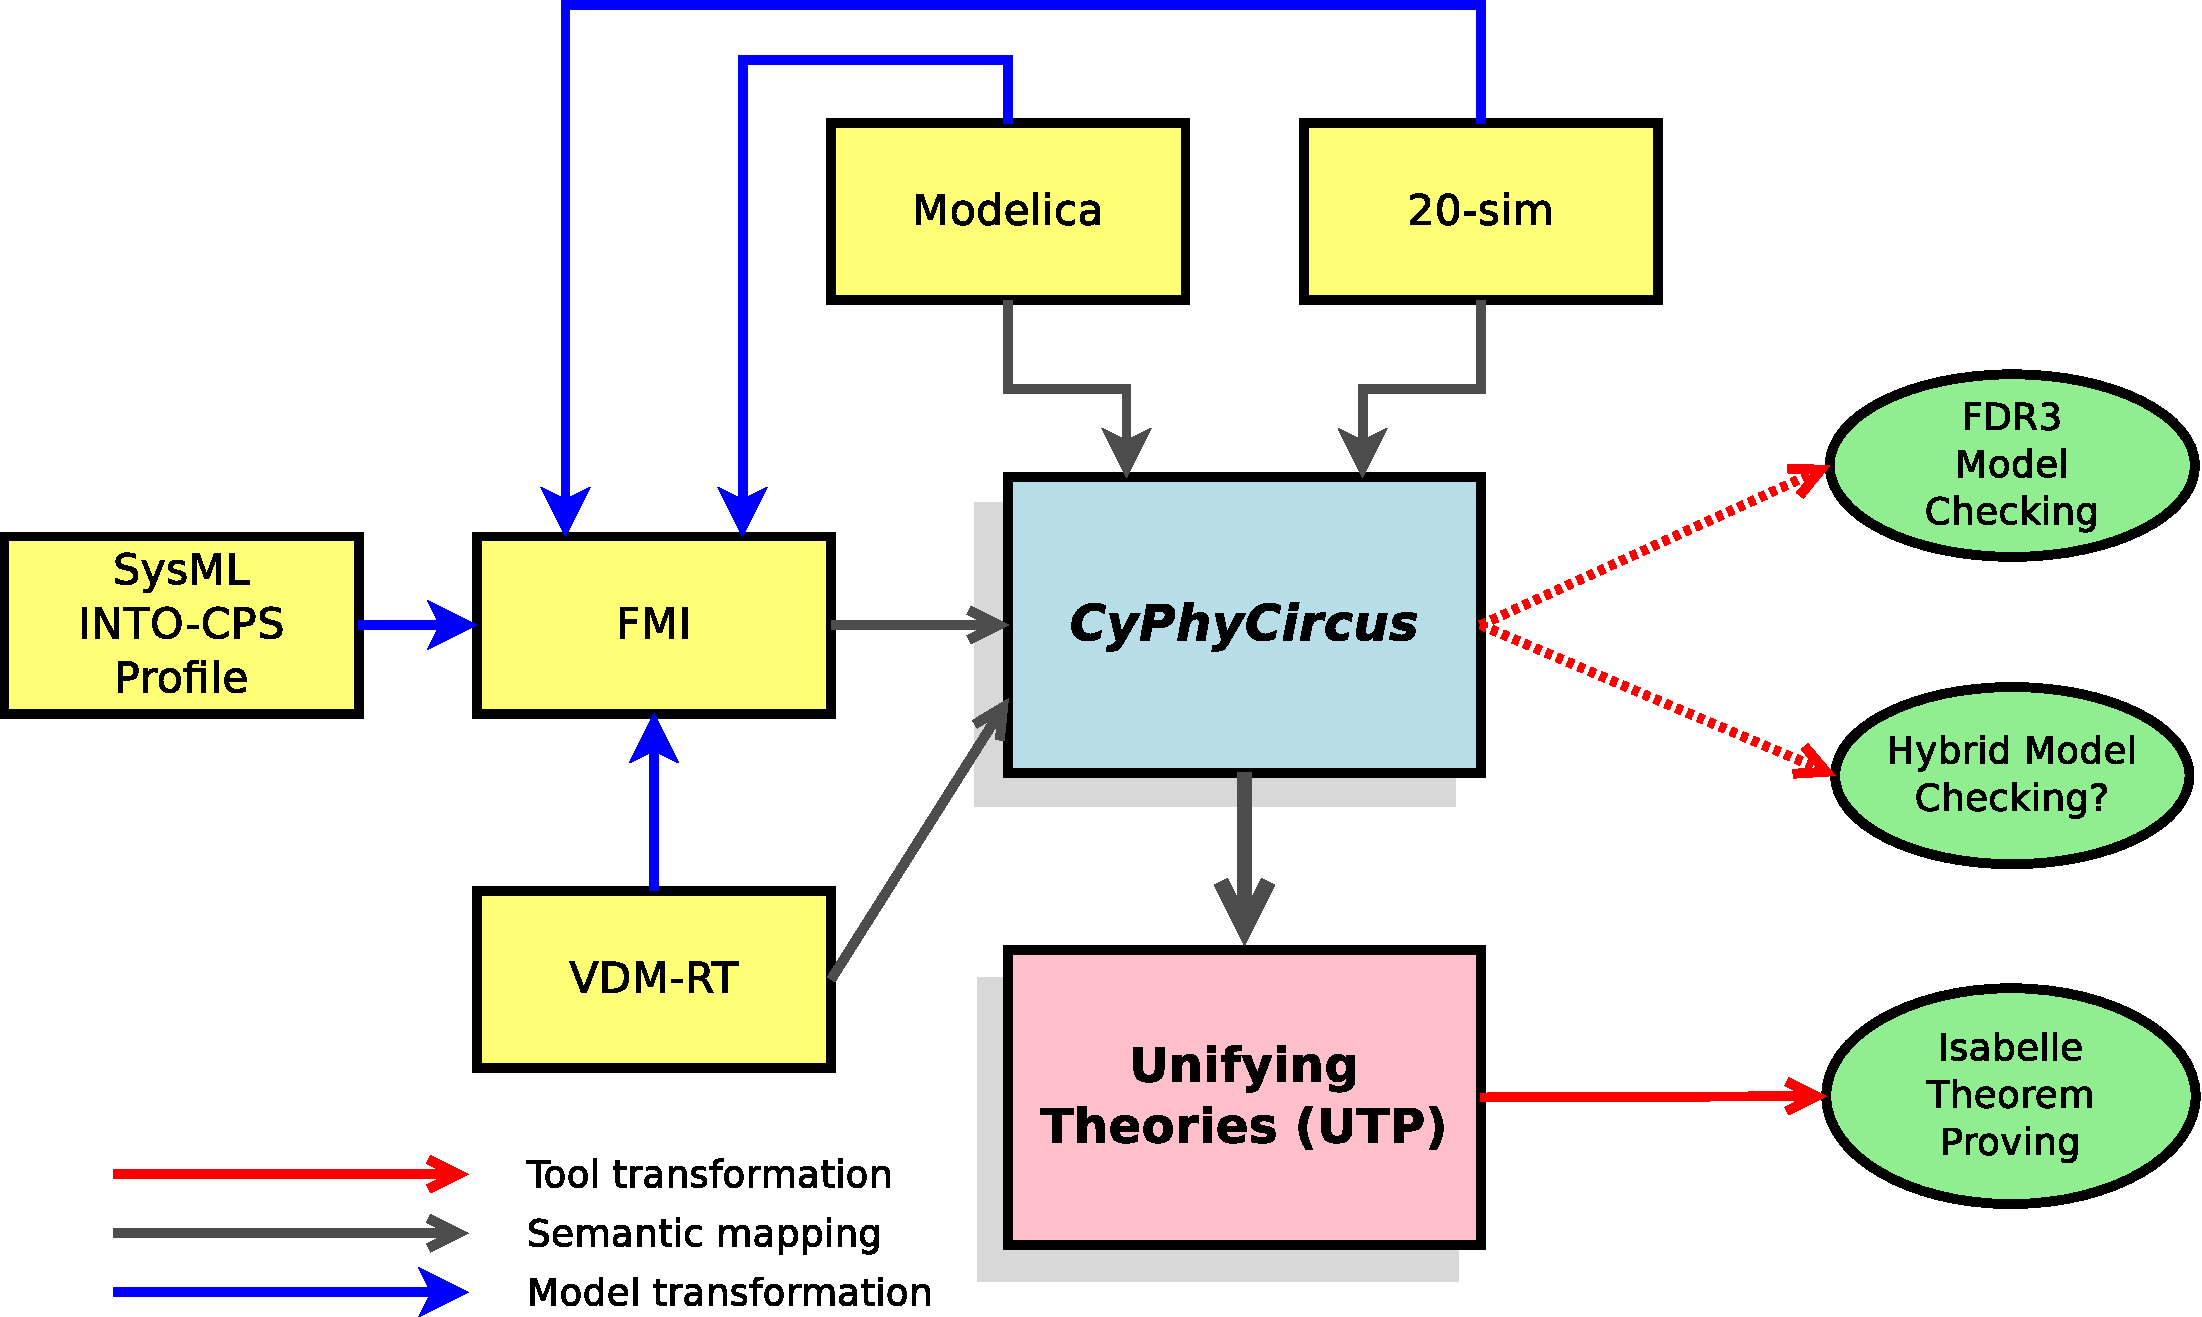
\includegraphics[width=14cm]{CyPhyCircus}
  \end{center}
  \caption{\CyPhyCircus as the INTO-CPS lingua franca}
  \label{fig:CyPhyCircus}
\end{figure}

\subsection{Functional Mock-up Interface}%

Because CPSs comprise both real-world entities and digital components, their modelling and designing typically requires a combination of different languages and tools that adopt complementary specification paradigms. For real-world artefacts, physics models in the form of differential equations are the norm. Digital components, such as software controllers, are typically described via control diagrams, state machines, and real-time programs. This diversity of specification and design methods makes CPS challenging to study and analyse.

Co-simulation~\cite{GomesTBLV2017} is perhaps the de facto technique for analysing the behaviour of CPS. It requires that models of artefacts are simulated in isolation, while master algorithms control the various simulators and thereby orchestrate the co-simulation as a whole. This raises issues of interoperability between the master algorithm and the simulators. The Functional Mock-up Interface (FMI) Standard~\cite{Blochwitz2011} has been proposed to alleviate those issues, and has since been successfully used in many industrial applications.  The FMI standard prescribes how master algorithms (MA) and simulators communicate. It does so using a bespoke API that simulators have to implement, and that can be used to devise compliant master algorithms. The API enables master algorithms to exchange data between the components of a co-simulation, called FMUs (Functional Mock-up Units), perform simulation steps, and suitably deal with errors in simulators. It also allows for advanced features such as roll-back of already performed steps.

While (co)simulation is currently the predominant approach to validate CPS models, the INTO-CPS approach uses a complementary technique based on a formal model of an FMI system. Our technique formalises both the master algorithm and the simulated FMUs, and allows for verification of their properties.

Whereas (co)simulation helps engineers to quickly gauge the implications of modelling and design decisions, our formal analysis has the potential to complement simulation with universal guarantees, both about the master algorithm and co-simulated system. The former is important since simulations depend on parameters and algorithms, and are software systems (with possible faults) in their own right. The latter is important since it is usually not possible to run an exhaustive number of simulation scenarios as a means of testing the system towards producing strong certification evidence.

For our formal modelling, we use Circus: a process algebra with added features for supporting stateful models. It has proved adequate and useful for modelling master algorithms~\cite{CavalcantiWA2016} due to its capabilities of capturing concisely the data and control aspects of such algorithms, including data exchange between the FMUs and their concurrent execution. Circus models can be subjected to verification techniques. These include both model-checking approaches~\cite{GrumbergV2008}, refinement~\cite{CavalcantiSW2003}, and (automatic) theorem proving~\cite{OliveiraCW2009}.

We use an abstract relational model of FMI co-simulations that focuses on the essence of the FMI computational paradigm [D2.3a]. We have  considered a concrete reactive model of FMI that faithfully models the FMI interface as well as master algorithms. This extends and elaborates the work in [D2.2c] by providing a comprehensive Circus model that has been mechanised in the theorem prover Isabelle/UTP~\cite{FosterZW2016}.

We have presented a complete and final Circus model of the FMI standard for co-simulation. To accomplish this, we have embedded the Circus language into Isabelle/UTP, allowing us to mechanise our FMI Circus model. In  [D2.3c], we illustrated the use of our mechanisation by applying it to one of the industrial INTO-CPS case studies (a railways system). 

For proof support, we pursue a technique, based on refinement, to show compliance of master algorithms with regards to the FMI standard~cite{Modelica2014}. Unlike other approaches, such as~\cite{Broman2013}, we can profit from high-level algebraic laws and a stepwise approach that culminates in executable code, for both the FMUs and master algorithm.

We have shown how our work completes the general reasoning technique presented in [D2.3a]. That technique proposes a refinement-based approach: we start with a discrete abstraction of a co-simulation that does not need to consider the master algorithm and is used to establish fundamental safety properties. Our work has filled an important gap: the transformation of an abstract FMU model into a concrete one that can be translated into code.

% References

% [Modelica2014] Modelica Association. Functional Mock-up Interface for Model Exchange and CoSimulation. Technical Report Document Version 2.0, Linköping University (Sweden), July 2014. Available from http:// fmi-standard.org/downloads/.
% [CavalcantiSW2003] A. Cavalcanti, A. Sampaio, and J. Woodcock. A Refinement Strategy for Circus. Formal Aspects of Computing, 15(2):146–181, November 2003.
% [CavalcantiWA2016] A. Cavalcanti, J. Woodcock, and N. Amalio. Behavioural Models for FMI Cosimulations. In Proceeings of ICTAC 2016, volume 9965 of Lecture Notes in Computer Science, pages 255–273. Springer, October 2016.
% [Broman2013] D. Broman et al. Determinate Composition of FMUs for Cosimulation. In Proceedings of EMSOFT 2013, pages 2:1–2:12. IEEE Press, September 2013.
% [Blochwitz2011] T. Blochwitz et al. The Functional Mockup Interface for Tool independent Exchange of Simulation Models. In Proceedings of the 8th International Modelica Conference, pages 105–114, March 2011.
% [FosterZW2016] S. Foster, F. Zeyda, and J. Woodcock. Unifying Heterogeneous StateSpaces with Lenses. In Proceedings of ICTAC 2016, volume 9965 of Lecture Notes in Computer Science, pages 295–314. Springer, October 2016.
% [GomesTBLV2017] C. Gomes, C. Thule, D. Broman, P. G. Larsen, and H. Vangheluwe. Cosimulation: State of the art. ArXiv e-prints, arXiv:1702.00686, February 2017.
% [GrumbergV2008] O. Grumberg and H. Veith. 25 Years of Model Checking: History, Achievements, Perspectives, volume 5000 of Lecture Notes in Computer Science. Springer, 2008.
% [OliveiraCW2009] M. Oliveira, A. Cavalcanti, and J. Woodcock. A UTP semantics for Circus. Formal Aspects of Computing, 21(1):3–32, February 2009.
